\section{Objective}

Phase 3 was performed to identify possible security weaknesses in
the OWASP Juice Shop application using automated scanning.

The main tool used in this phase was OWASP ZAP. The scan was used to
find potential vulnerabilities that required further testing.

The alerts generated during this phase were treated as potential
findings. They were not considered confirmed vulnerabilities until
they were manually tested in Phase 4.

\section{Scanning Methodology}

The following scanning activities were performed using OWASP ZAP:

\begin{enumerate}

    \item \textbf{Spider Scan} -- The traditional Spider was used to
    crawl the application and discover available pages, links, and
    endpoints.

    \item \textbf{AJAX Spider} -- The AJAX Spider was used because
    Juice Shop is a JavaScript-based application. It helped discover
    additional pages and content that may not be found by the
    traditional Spider.

    \item \textbf{Passive Scan} -- ZAP analyzed the traffic generated
    during browsing and crawling. This helped identify common
    security issues without actively attacking the application.

    \item \textbf{Active Scan} -- ZAP actively tested the discovered
    application endpoints for possible vulnerabilities, including
    SQL Injection, Cross-Site Scripting, and other web security
    issues.

    \item \textbf{Alert Review} -- The alerts generated by ZAP were
    reviewed and compared with the application's actual behavior.
    Findings that required further testing were carried forward to
    Phase 4 for manual validation.

\end{enumerate}

\section{ZAP Scan Evidence}

The following evidence shows the OWASP ZAP alerts identified during
the scanning process for the two findings that were flagged by
automated scanning: SQL Injection (SQLI-02) and Open Redirect (OR).

\begin{figure}[H]
    \centering
    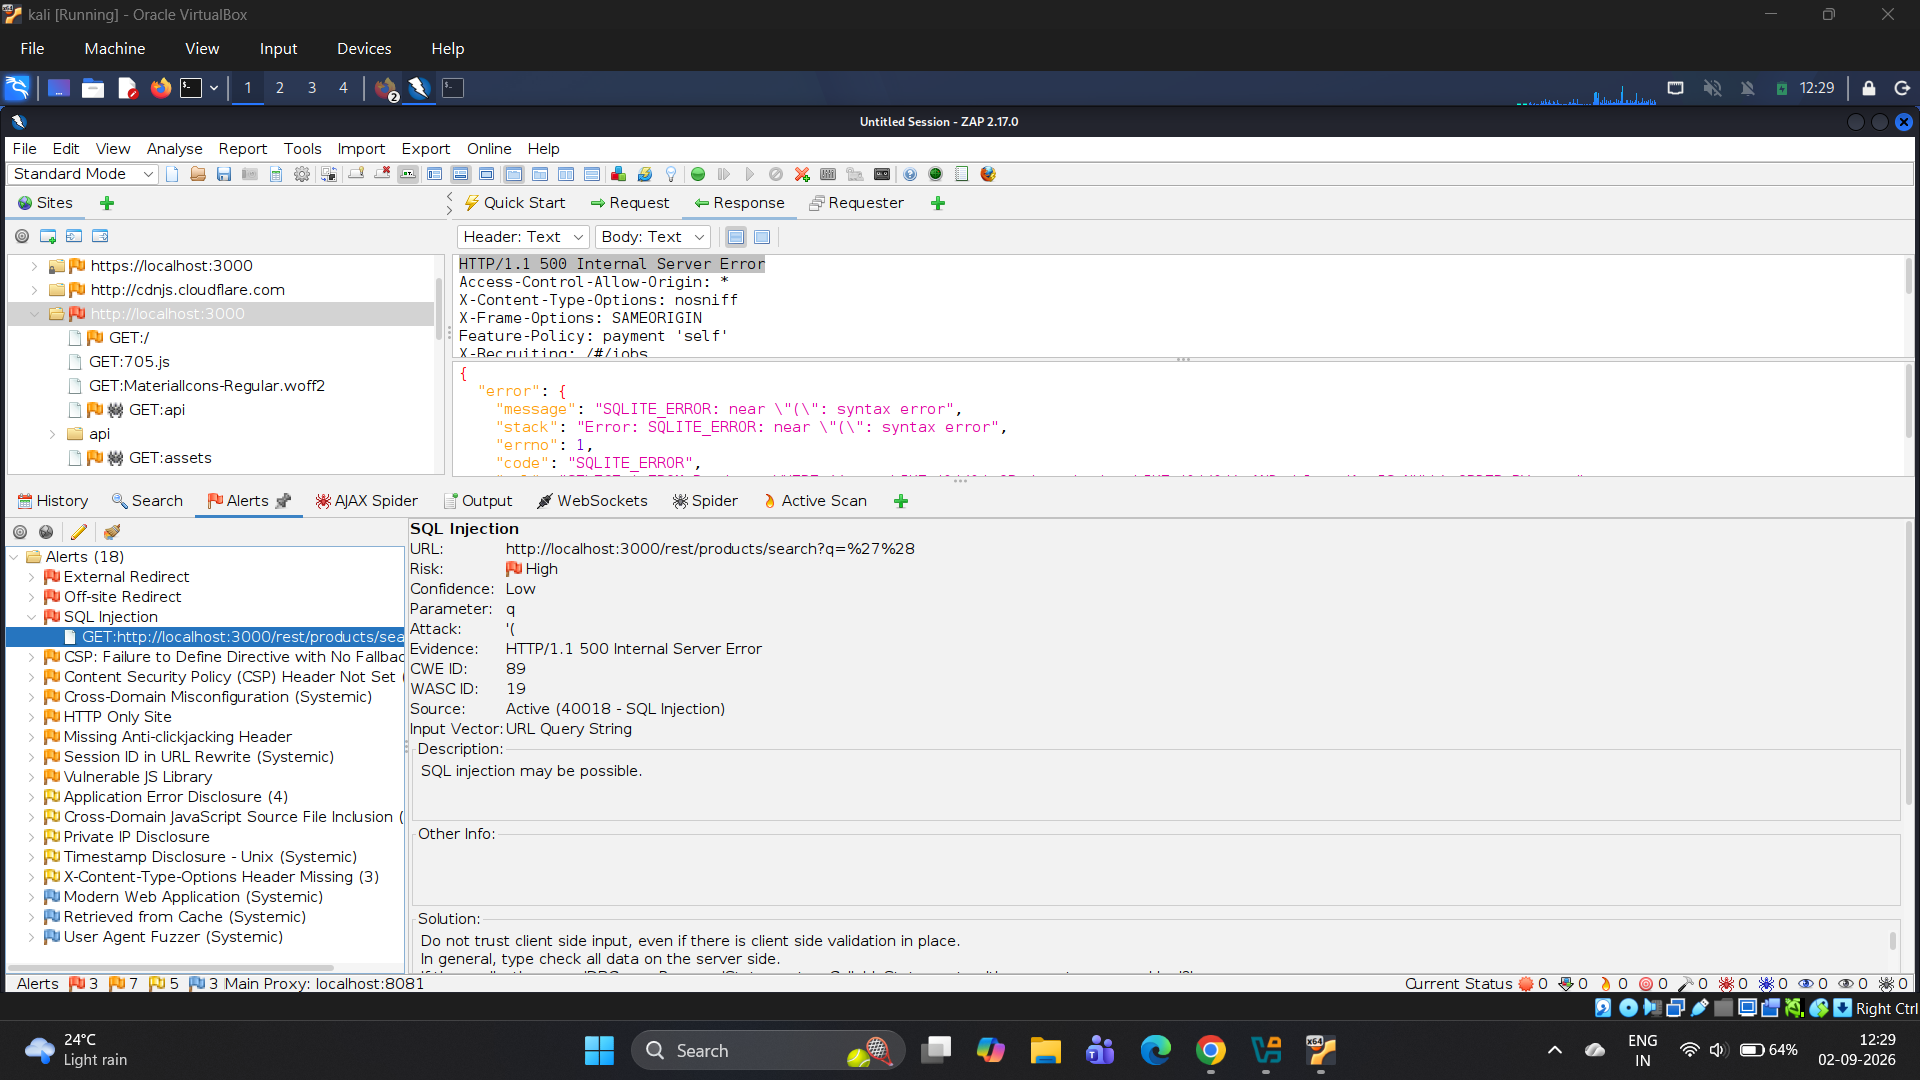
\includegraphics[width=0.8\textwidth]
    {evidence/phase3/zap/sqli02-01-zap-alert-detection.png}
    \caption{OWASP ZAP identifying a possible SQL Injection vulnerability
    in the product search parameter}
    \label{fig:zap-sqli02}
\end{figure}

\begin{figure}[H]
    \centering
    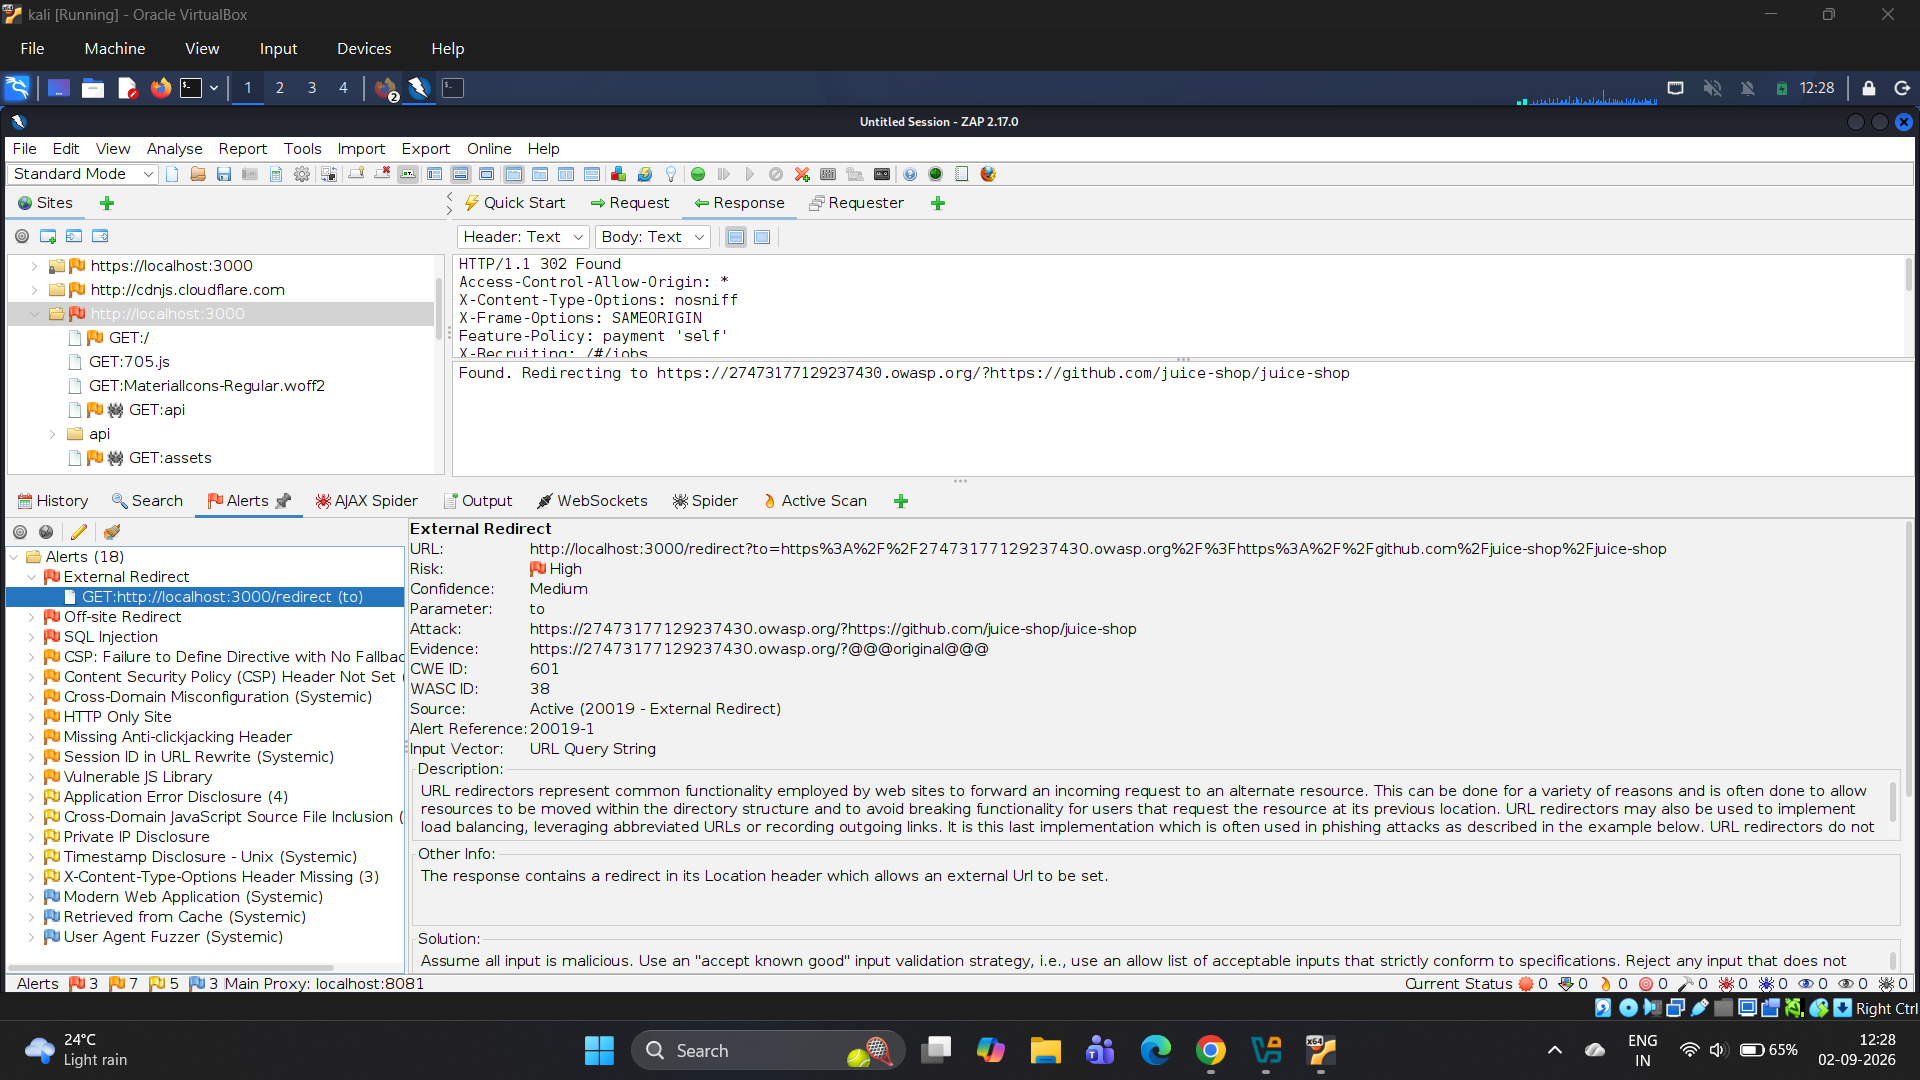
\includegraphics[width=0.8\textwidth]
    {evidence/phase3/zap/openredirect-01-zap-alert-detection.png}
    \caption{OWASP ZAP identifying a possible Open Redirect
    vulnerability in the redirect parameter}
    \label{fig:zap-or}
\end{figure}

Both alerts shown above were treated as potential vulnerabilities.
Further testing was performed in Phase 4 using Burp Suite (and
SQLMap for SQLI-02) to confirm each issue and determine its actual
impact. Full exploitation details are provided in
Sections~7.4 and~7.7.

\section{Scan Results}

The OWASP ZAP scan generated a total of 18 alerts.

The alerts were reviewed before deciding which issues required
detailed manual testing. An alert from an automated scanner does not
always mean that a real vulnerability exists. Therefore, the findings
were manually tested before being included as confirmed
vulnerabilities in this report.

\begin{table}[H]
\centering
\begin{tabular}{|l|l|}
\hline
\textbf{Scan Result} & \textbf{Count} \\
\hline
Total ZAP Alerts & 18 \\
\hline
Findings Selected for Phase 4 Validation & 2 \\
\hline
Other Alerts Not Carried Forward & 16 \\
\hline
\end{tabular}
\caption{Summary of OWASP ZAP scan results}
\end{table}

\section{Findings Selected for Manual Validation}

The following two findings were identified through automated
scanning and selected for further testing and evidence collection in
Phase 4:

\begin{table}[H]
\centering
\begin{tabular}{|l|p{8cm}|}
\hline
\textbf{Finding ID} & \textbf{Vulnerability} \\
\hline
SQLI-02 & SQL Injection -- Product Search Parameter \\
\hline
OR & Open Redirect -- Unvalidated Redirect Parameter \\
\hline
\end{tabular}
\caption{Findings selected for Phase 4 validation (ZAP-detected)}
\end{table}

The remaining confirmed findings -- BAC, IDOR, AUTH,
SQLI-01 (Authentication Bypass through Login), XSS, and CSRF --
were not flagged by the OWASP ZAP automated scan and were instead
identified through manual testing during Phase 4, as documented in
their respective finding sections.

\section{Phase 3 to Phase 4}

Phase 3 was mainly used for automated discovery. The alerts provided
an initial indication of possible security weaknesses for two of the
eight confirmed findings.

In Phase 4, both the ZAP-flagged findings and the additional
manually-identified findings were tested and confirmed using Burp
Suite and other appropriate tools. Evidence was collected to prove
whether each issue was actually exploitable and to understand its
security impact.

Therefore, the report follows this process:

\begin{center}
\textbf{Automated Scanning / Manual Discovery}
$\rightarrow$
\textbf{Alert Review}
$\rightarrow$
\textbf{Manual Validation}
$\rightarrow$
\textbf{Evidence Collection}
$\rightarrow$
\textbf{Confirmed Finding}
\end{center}

\section{Note}

The detailed technical information and exploitation evidence for the
confirmed vulnerabilities are provided in the Phase 4 finding
chapters.

The purpose of Phase 3 is to document how potential vulnerabilities
were discovered, while Phase 4 provides the detailed proof and impact
of the confirmed vulnerabilities.